
Let,
\begin{align}
\vec{A}&=a\myvec{\cos\theta\\ \sin\theta},\vec{B}=\myvec{0\\0},\vec{C}=\myvec{a\\0} \\
    &= 5.5\myvec{\cos60\degree\\\sin60\degree},\vec{B}=\myvec{0\\0},\vec{C}=\myvec{5.5\\0}
    \end{align}
after substituting     $\theta=60\degree$
and $a=5.5$.  The triangle is then plotted in Fig. \ref{constr/tri/11/fig:triangle ABC}
%
\begin{figure}[ht]
\centering
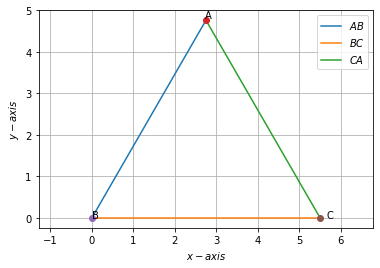
\includegraphics[width=\columnwidth]{solutions/triangle/11/Figure 1.png}
\caption{$\triangle ABC$}
\label{constr/tri/11/fig:triangle ABC}
\end{figure}
